\documentclass[DM,lsstdraft,toc]{lsstdoc}
\usepackage{graphicx}
\usepackage{url}
\usepackage{latexsym}
\usepackage{color}
% black, blue, brown, cyan, darkgray, gray, green, lightgray, lime, magenta, blue, orange, pink, purple, red, teal, violet, white, yellow.
\usepackage{enumitem}

\title[LSST Special Programs]{Data Management \\ and LSST Special Programs}

\author{M.~L.~Graham, M.~Juri\'{c}, and E.~Bellm}

\setDocRef{DMTN-nnn}
\date{\today}
\setDocRevision{TBD}
\setDocStatus{draft}

\setDocAbstract{\textbf{WORKING DRAFT (contains rough notes and partial thoughts) } but intended to be an overview of any and all potential requirements on data management (DM) from Special Programs such as the deep drilling fields (DDF) or mini-surveys. We also summarize the plans for how the Special Programs data will be integrated into the wide-fast-deep (WFD) Main Survey data products(Levels 1 and 2). It is the intent that this document evolve to become an internal catalog of change requests to the DM Level 1 and 2 pipelines and products, and a community resource for future Special Program white papers and preparations for Level 3 pipelines.}


\setDocChangeRecord{%
\addtohist{1}{2017-04-??}{Internal working document.}{Melissa Graham}
%\addtohist{2}{yyyy-mm-dd}{Future changes}{Future person}
}

\begin{document}

\maketitle

% CITATION EXAMPLES
% \verb|\citellp|: \citellp{LPM-17, LSE-30} \\
% \verb|\citell|: (SRD; \citell{LPM-17,LSE-29}) \\
% \verb|\citep[][]|: \citep[e.g.,][are interesting]{LPM-17,LSE-29} \\
% \verb|\cite|: \cite{LPM-17,LSE-29}



% % % % % % % % % % % % % % % % % % % % % % % % % % % % % % % % % % % % 
\section{Introduction} \label{sec:intro}

The intent of LSST DM for processing data from Special Programs can be summarized by the following statement, which reflects Section 6 of the Data Products Definitions Document (DPDD, LSE-163, \cite{LSE-163}):

\vspace{-20pt}
\begin{quote}
LSST will not write unique algorithms for processing Special Programs data or reprocessing Main Survey data, but LSST will reconfigure the pipelines and generate imaging and catalog products for Special Programs data whenever possible, and LSST will make its codes accessible to the science community and commit $\sim$10\% of its computing resources toward enabling Level 3 analysis and data product creation, including user-driven Special Programs processing.
\end{quote}

\noindent The purpose of this study is to ensure that the requirements and plans of DM, as written down in all major DM documentation, accurately reflects this intent. In particular, this study is designed to review: \\
(1) the processing and products that are required to enable science for Special Programs, \\
(2) the current plans for DM processing and products with respect to Special Programs, \\
(3) whether the DM plans meet the expected needs of Special Programs, and \\
(4) any necessary changes to be written into the requirements, designs, and plans.

\noindent The concerns raised by this study fall into three main categories: \\
(1) Whether DM will be able to process the full diversity of non-standard visit images, and if not, what the boundaries will be. \\
(2) Ensuring that DM's intent to process Special Programs data with reconfigured pipelines and provide separate data products that meet the science goals of each program is accurately reflected in all documents, as it is in the DPDD. \\
(3) Clarifying the computational sizing plans for processing and storage of Special Programs data and whether it is this separate from the allocation for end-user Level 3 analysis.



% % % % % % % % % % % % % % % % % % % % % % % % % % % % % % % % % % % % 
\section{The Potential Diversity of Special Programs Data} \label{ssec:data}

To better identify what might be missing in the DM plan to accommodate Special Programs, we need a comprehensive understanding of the potential diversity in future Special Programs data. The concern is that if Special Programs data is significantly different from the Wide-Fast-Deep survey of tiled, nighttime, 15--30 second exposures (standard visit images), then it might not be adequately handled by the DM system. To get a handle on the potential diversity of Special Programs data, we first attempt to understand the technical limitations that the facility and instrumentation places on the observing modes, e.g., exposure times, filter changes (Section \ref{ssec:data_bounds}). Next, we explore the current set of proposed science programs for LSST (Section \ref{ssec:data_science}) and the types of observations they would want to do, and then describe when and how we can incorporate revisions to these proposals from the user community in the future (Section \ref{ssec:data_comm}). Finally, we explore whether DM can or should set down any technical constraints on how far an observing program can deviate from a sequence of standard visit images and still be processed by DM pipelines, be they the reconfigured and/or the standard Level 1 and 2 pipelines (Section \ref{ssec:data_DMconstraints}).


% % % % % % % % % % % % % % % % % % 
\subsection{Observing Boundaries for Special Programs}\label{ssec:data_bounds}

We can constrain the potential diversity of Special Programs data if we know the observing boundaries that will be imposed on the accepted proposals. So far, only one aspect of the LSST Special Programs are set: the locations of the four chosen deep drilling fields\footnote{\url{https://www.lsst.org/scientists/survey-design/ddf}}. \cite{2008arXiv0805.2366I} describes a nominal DDF data set as e.g., a series of fifty 15 second exposures in each of the $griz$ filters obtained once every two nights for four months, which would yield a nightly stack depth of $r<26.5$ and a full stack depth of $r<28.0$ (once combined with the wide-fast-deep survey data). Additionally, three mini-survey areas that have already been considered in detail are likely to move forward: the North Ecliptic Spur (NES), the South Celestial Pole, and the Galactic Plane (see Figure 8 of \cite{2008arXiv0805.2366I}). We have a summary collection of past white papers and informally proposed mini-surveys in Section \ref{ssec:data_science}.

All other aspects of LSST Special Programs remain open to proposals, including: \\
$\bullet$ additional deep drilling fields \\
$\bullet$ refined observing strategies for deep drilling fields \\
$\bullet$ optimized survey areas for the NES, South Pole, and Galactic Plane \\
$\bullet$ refined observing strategies for the NES, South Pole, and Galactic Plane \\
$\bullet$ additional mini-surveys \\
$\bullet$ the total fraction of time spent on Special Programs (nominally 10\%)

There will be some technical limitations on the mini-surveys that will be possible. Here's a rough draft list of such potential issues. It is not the job of this document to define the camera/observatory technical boundaries, but we do need to know what they are in order to predict the diversity of incoming data that DM will be processing. This list will be updated in the future (or revised to point to where these boundaries are defined). In Section \ref{sssec:dmplans_review_oss}, as we review the Observatory System Specifications (OSS, LSE-30, \cite{LSE-30}) document we highlight a couple more questions regarding potential boundaries on Special Programs observations.

Filter Changes (and see \ref{OSS-6}): \\
$\bullet$ The maximum time for filter change is 120 seconds: 30 seconds for the telescope to reorient the camera to its nominal zero angle position on the rotator, and 90 seconds to the camera subsystem for executing the change (OSS-REQ-0293). \\
$\bullet$ \textit{(MLG - The next three points are from a document-in-progress by Ivezic and Ritz; update to formal citation when it's public-facing.)} \\
$\bullet$ The minimum time between filter changes has no restrictions from e.g., thermal tolerances. However, based on overheads and efficiency, it is recommended to keep the filter change rate lower than once every 10 minutes. \\
$\bullet$ The maximum total number of filter changes is 100,000 over 15 years, an average of 18 changes per night. \\
$\bullet$ The maximum number of filter swaps in/out of the carousel is 3000 in 15 years, or once every two nights.

Exposure Times (and see \ref{OSS-5}): \\
$\bullet$ The minimum exposure time is 1 second, with a stretch goal of 0.1 seconds (OSS-REQ-0291). \\
$\bullet$ The maximum exposure time is not restricted. \\
$\bullet$ However, for exposure times there are other considerations. The minimum exposure time needed to create an image with a PSF that is well-formed enough for difference imaging is a separate question. Changing the exposure time also affects the photometric and astrometric calibrations. Assuming a 1 second exposure can be reduced and calibrated, its detected point sources will span $13 < r < 21$ magnitudes, whereas a 15 second exposure saturates at $r\sim15.8$ mag. A 150 second image would saturate at $r\sim18.3$, perhaps leaving too few stars overlapping with e.g., templates or WFD images, for astrometric and photometric calibrations. Additionally, the impact on CR rejection routines is untested for long exposures. 

Camera Rotation (and see \ref{OSS-7}): \\
$\bullet$ \textit{MLG - I heard there might be a lifetime maximum on the rotator, such that if a mini-survey wants to jump between patches that are far apart on the sky repeatedly, that could wear out the mechanism? Can't remember where I heard it.}

Telescope Slews: \\
$\bullet$ \textit{MLG - Obviously, long slews would cause additional overheads and a loss of observing efficiency, but are there other limitations?}

Calibration Images (and see \ref{OSS-2}, \ref{OSS-4}): \\
$\bullet$ The necessary afternoon calibrations for a Special Program must fit into some amount of time left over after the WFD main survey daily calibration frames are obtained.

Operations Simulations: \\
$\bullet$ Mini-survey observing strategies will have to show that they do not negatively impact the LSST's ability to complete the wide-fast-deep survey; not necessarily in the next call for white papers, but later during the review and revise stage, once the new OpSim runs incorporating proposed mini-surveys have been generated.

Total Time: \\
$\bullet$ It has been regularly stated that 10\% of the total observing time will be used for special programs (90\% goes to the WFD main survey), but this could be changed if significant science is enabled. \\



% % % % % % % % % % % % % % % % % % 
\subsection{Currently Proposed Special Programs} \label{ssec:data_science}

In this section we compile information about the science goals and observational methods for Special Programs that have already been proposed. We use these to infer the potential deviations from standard visit images, and to get a basic idea of the DM processing needs that would be required to enable the science; this Section is mainly descriptive and we do not spawn any {\bf Concerns} here. In Section \ref{sec:SPCS}, we create much more detailed DM Processing Case Studies for several of these Special Programs in order to identify any potential issues with reconfiguring the DM pipelines to create specific data products for these programs; any {\bf Concerns} that arise are detailed in that section. Below, we list the set of resources that we used to compile this information, and in Table \ref{tab:ddfms} we list the four extragalactic deep drilling fields have already been specified along with an {\it incomplete} list of potential mini-surveys that people are thinking about (mainly from the presentations of Brandt and Ridgway at the 2016 AHM).

\noindent {\bf Resources:} \\
$\bullet$ ``LSST: from Science Drivers to Reference Design and Anticipated Data Products" Ivezi\'{c} et al. (2008), \cite{2008arXiv0805.2366I} \\
$\bullet$ The LSST Science Requirements Document (SRD), LPM-17, \cite{LPM-17} \\
$\bullet$ LSST Deep Drilling white papers from 2011: \url{https://project.lsst.org/content/whitepapers32012} \\
$\bullet$ ``General Review of the Proposed DDF and MS", LSST AHM Aug 2016 presentation by Niel Brandt \url{https://project.lsst.org/meetings/lsst2016/sites/lsst.org.meetings.lsst2016/files/Brandt-DDF-MiniSurveys-01.pdf} \\
$\bullet$ ``Simulations, Metrics and Merit Function for Mini-Surveys and DDF", LSST AHM Aug 2016 presentation by Stephen Ridgway \url{https://project.lsst.org/meetings/lsst2016/sites/lsst.org.meetings.lsst2016/files/Ridgway-SimulationsMetrics_1.pdf} \\
$\bullet$ ``LSST's DC [Deep CoAdd] Bias Against Planets and Galactic-Plane Science" by A. Gould, \cite{2013arXiv1304.3455G} \url{https://arxiv.org/abs/1304.3455} \\
$\bullet$ Chapter 10 ``Special Surveys" of the Observing Strategy White Paper \cite{2017arXiv170804058L}

\begin{table}[h]
\begin{center}
\begin{footnotesize}
\caption{Approved DDF and Incomplete List of Potential MS.}
\label{tab:ddfms}
\begin{tabular}{lll}
\hline \hline
Name & Coordinates & Description  \\
\hline
DDF Elias S1    & 00:37:48, -44:00:00  & approved, cadence TBD \\
DDF XMM-LSS & 02:22:50, -04:45:00  & approved, cadence TBD  \\
DDF Extended Chandra Deep Field-South & 03:32:30, -28:06:00  & approved, cadence TBD  \\
DDF COSMOS  & 10:00:24, +02:10:55 & approved, cadence TBD  \\
DDF TBD  & & TBD \\
North Ecliptic Spur      & & solar system objects (find and characterize) \\
Galactic Plane             & & more intensive stellar surveying \\
South Equatorial Cap  & & S/LMC and more Galactic science \\
Twilight                        & & short exposures (0.1s) for bright stars \\
Mini-Moons                     &  & finding mini-moons \\
Sweetspot                       & & 60 deg from Sun for NEOs on Earth-like orbits \\
Meter-Sized Impactors     & & detection a week before impact \\
GW Optical Counterparts & & search and recovery \\
Old Open Cluster M67      & dec +12 & compact survey above Galactic plane  \\
\hline
\end{tabular}
\end{footnotesize}
\end{center}
\end{table}

\textbf{A Nominal DDF Observing Strategy -- } Ivezi\'{c} et al. (2008, \cite{2008arXiv0805.2366I}), Section 3.2.1 ``Mini-Surveys": describes a nominal DDF data set as $\sim50$ consecutive $15$ second exposures in each of four filters in one hour per night, once every two nights, for four months. Each observation would have a limit of $r\sim24.5$; a one-hour nightly stack would have a limit of $r\sim26.5$; and and assuming a $60\%$ completion rate (weather), the four-month $\sim40$ hours stacked together with the $\sim180$ main survey visits would yield a limit of $r\sim28$. 

\medskip
\noindent \textbf{Solar System Objects (SSO)}\\
$\bullet$ North Ecliptic Spur: observations in this area of the sky will yield more $\geq140$ m near-earth objects (NEOs) for the final LSST sample (Brandt talk). \\
$\bullet$ Mini-Moons: finding and studying temporarily captured satellites of the Earth. (Section 10.2, \cite{2017arXiv170804058L}) \\
$\bullet$ Sweetspot: use twilight fields to find NEOs in Earth-like orbits (never in opposition fields). (Section 10.2, \cite{2017arXiv170804058L}) 
$\bullet$ Meter-Sized Impactors: finding and tracking meter-sized impactors $<2$ weeks before impact.  (Section 10.2, \cite{2017arXiv170804058L}) \\
$\bullet$ Detecting faint SSO down to $r\sim27$ would be done by applying shift-and-stack (SAS) processing to a mini-survey data of standard visit images (faint SSO include: Trans-Neptunian Objects Trojans, asteroids, long-period comets, dwarf planets) \citep{BeckerWP}. Regarding SAS, \cite{BeckerWP} says that ``the multi-fit algorithm ... naturally provides a base infrastructure for this process. In particular, the marshaling of the pixels to attempt a given photometric measurement is non-trivial when tens of thousands of images are required. However, the multi-fit middleware is required to do exactly this, so we expect that this issue will be resolved by the time SAS is needed." \\
$\bullet \bullet \bullet$ {\bf Summary.} Most of these science goals can be achieved with standard visit images obtained in a normal survey pattern taken during the night. The exception is a Sweetspot survey, which occurs during twilight and thus may require shorter exposures. Many of these science goals will also be possible by using the products of Moving Object Processing System (MOPS), which runs on the Level 1 {\tt DIASource} catalogs updated each night. The exception is finding faint SSOs through shift-and-stack processing; SAS is not a capability of the DM system, cannot be done solely by reconfiguring DM pipelines, and is therefore considered Level 3. See Sections \ref{ssec:SPCS_SAS} and \ref{ssec:SPCS_MM} for more detailed DM processing case studies.

\noindent \textbf{Stars in the Milky Way and Magellanic Clouds} \\
$\bullet$ When surveying the Galactic Plane, obtaining all the images over a short time span would mitigate proper motion loss (and increase flare detection rates) and help identify useful stellar populations. When targeting Galactic plane regions and/or open clusters, typically 1 to 3 filters are needed for detections of e.g., faint stars already detected in $z$ and $y$ but needing $i$ to distinguish from red galaxies \cite{DhitalWP}. \\
$\bullet$ A nominal deep-drilling observing strategy over the full L/SMC galaxies will characterize stellar variability to $M_V<6.5$ on timescales from 15s to 3d \cite{SzkodyWP}. For this, special co-adds may be required, e.g., {\it "to reach variability levels of 0.1 to 0.005 mag will require co-adds depending on the timescale of the particular variables"}. \citep{SzkodyWP}. \\
$\bullet$ A Twilight Short Exposure survey would enable bright stars, which have longer monitoring baselines due to historical observations, to be put on the same photometric system as the deeper LSST WFD main survey catalog. \\
$\bullet$ A short-exposure survey of M67, Chapter 10.4 of \cite{2017arXiv170804058L}, suggests using the stretch goal of 0.1 second exposures or, if that is not possible, {\it ``custom pixel masks to accurately perform photometry on stars as much as 6 magnitudes brighter than the saturation level"}. \\
$\bullet \bullet \bullet$ {\bf Summary.} Many of these science goals can be achieved with standard visit images, but with alternative observing strategies such as limiting the number of filters or concentrating the depth build-up into shorter timeframes; the exception is short-exposure surveys to obtain bright stars. Similarly, most of these science goals can be met by reconfiguring the planned DM pipelines to detect sources, measure proper motion, and create deep stacks. The exception might be in processing exposures as short as 0.1 seconds, and attempting to measure flux of a saturated stars. See Sections \ref{ssec:SPCS_GPVSEx} and \ref{ssec:SPCS_M67} for more detailed DM processing case studies.

\noindent \textbf{Exoplanets} \\ 
$\bullet$ Transits. The nominal DDF plan described in \cite{2008arXiv0805.2366I} would allow for $1\%$ variability detection over hour-long timescales, which is suitable for detecting transits. A DDF field at Galactic latitude $30$ degrees would yield $10^6$ stars at $r<21$ that would have ${\rm SNR}>100$ in each single exposure of the sequence (as described in Section 3.1.2 of \cite{2008arXiv0805.2366I}). \cite{2013arXiv1304.3455G} describes how transits can be extract from a wider-area survey of the Galactic Plane.\\
$\bullet$ Microlensing.  Slower than a transit, \cite{2013arXiv1304.3455G} suggests that $\sim22$ mag imaging over the Galactic Plane region every 3-4 days (i.e., the WFD nominal cadence) can find microlensing candidates, which would then need follow-up with external facilities. However, this will require image differencing in crowded fields. \cite{2013arXiv1304.3455G} suggests that the Galactic Plane can yield a lot of science despite the fact that its eventual deep co-adds would be uselessly confusion limited, and therefore should not be skipped. Microlensing can also be done with DDF-style observing at low Galactic latitudes. \\
$\bullet \bullet \bullet$ {\bf Summary.} All of these science goals appear possible with standard visit images. They might be possible with reconfigured DM pipelines, but this depends heavily on performance in crowded fields. See Section \ref{ssec:SPCS_GPVSEx} for a more detailed DM processing case study for Galactic Plane regions.

\noindent \textbf{Supernovae} \\
$\bullet$ The nominal DDF plan described in \cite{2008arXiv0805.2366I}, which builds nightly stacks with a limit of $r\sim26.5$ out of standard visit images, would extend the SN sample to $z\sim1.2$ and provide more densely sampled light curves for cosmological analyses. The optimal exposure time distribution might be 6, 5, 10, 10, 9, 10 in $ugrizy$. \cite{KesslerWP} \\
$\bullet$ High-cadence observations of DDF would be the only way to detect fast transients, particularly extragalactic novae, some tidal disruption events, optical counterparts to gamma-ray bursts, and peculiar SNe \cite{2014ApJ...794...23D}. \\
$\bullet$ Generating the best-possible individual SN light curves for cosmological analyses requires building special, deep-as-possible, SN-free host galaxy images and using them as a template. This will also be necessary for studying SNe that appear in the template image; i.e., that last $>1000$ days. These are mostly Type IIn, probably explosions of massive stars into dense circumstellar material, which are not used for cosmology but rather to study late-stage stellar evolution and mass loss. SN-free images will also be needed to measure correlated properties for cosmology and to do host-galaxy science. The latter, specifically the ``characterization of ultra-faint SN host galaxies", is also mentioned in the Galaxies DDF WP \cite{FergusonWP}. \\
$\bullet$ \textit{MLG - I'm not sure this has been yet proposed, but short-exposure observations to include nearby SNe on the same photometric system could be useful?} \\
$\bullet \bullet \bullet$ {\bf Summary.} All of these science goals appear possible with standard visit images (with the exception of an as-yet unproposed target-of-opportunity survey to obtain photometry for nearby, saturated SNe). Additionally, all are accessible with reconfigured DM pipelines to stack and difference the data. In particular, the Level 2 DRP codes to create ``transient-free CoAdds" will be suitable for generating the SN-free templates for DDF, as they will do for the Main Survey images. See also Section \ref{ssec:SPCS_SNDDF} for a DM processing case study to find SNe in a DDF.

\noindent \textbf{Galaxies} \\
$\bullet$ Use the additional depth of a DDF to build a large collection of low-$\mu$ objects. \cite{FergusonWP} mentions ``identification of nearby isolated low-redshift dwarf galaxies via surface-brightness fluctuations" and ``characterization of low-surface-brightness extended features around both nearby and distant galaxies". \\
$\bullet$ The DDF stacks can also be used to characterize of high-$z$ clusters, although this ability might depend on deblending extended objects. \\
$\bullet$ The DDF observations, when combined with the WFD, allow for AGN monitoring on a variety of timescales in well-characterized galaxies \citep{FergusonWP,GawiserWP}. \\
$\bullet \bullet \bullet$ {\bf Summary.} As with the SN science goals, these use standard visit images and reconfigured DM pipelines to make deep CoAdds and extract sources. In addition, it seems likely that Level 3 algorithms that are optimized to detect and characterize particular types of faint extended sources will be needed, but these are beyond the scope of DM. 

\noindent \textbf{Weak Lensing} \\
$\bullet$ The deeper imaging from DDFs can help with shear systematics and the effects of magnification in the analysis of WFD data (community forum, Jim Bosch) \\
$\bullet$ {\it Jim Bosch -- ``Will need to process at least some deep drilling fields (high-latitude ones) in the same way we process a full data release production before running the full data release production, so we can use the results to build priors and/or calibrate shear estimates on the wide survey"} ({\tt \Large{Community}} forum) \\
$\bullet$ {\it Jim Bosch -- ``Will need to process various wide-depth subsets of some deep drilling fields (again, high-latitude ones) using the regular DRP pipeline. We'll definitely want best-seeing, worst-seeing, and probably a couple of independent typical-seeing subsets, but there may be other ways we'd want to subdivide as well."} ({\tt \Large{Community}} forum)  \\
$\bullet$ {\it MLG side note -- Photo-$z$ are very important to weak lensing \citep{MaWP} and so perhaps the implemented method should be chosen with weak lensing science prioritized.} \\
$\bullet \bullet \bullet$ {\bf Summary.} As with the SN and Galaxies DDF-related science goals, these use standard visit images and reconfigured DM pipelines can be used to make deep CoAdds and extract sources, as Jim notes. 


% % % % % % % % % % % % % % % % % % 
\subsection{Future Input from Data Rights Holders} \label{ssec:data_comm}

Community input on LSST Special Programs will be ingested through a formal call for white paper proposals (Section \ref{sssec:data_comm_call}). This call will request that these white papers include a section that describes the processing needs that will enable their science goals; examples of processing case studies for some proposed Special Programs are given in Section \ref{sec:SPCS}. The DM team will also interact informally with the community through, e.g., a {\tt \Large{Community}} forum (Section \ref{sssec:data_comm_forum}) and might learn about users needs for DM processing through that means.

\subsubsection{Call for White Paper Proposals}\label{sssec:data_comm_call}

The document "Cadence Exploration and Improvement Plan" (by Zeljko, Lynne, Andy) proposes that the next call for DDF White Papers (proposed fields and cadences) be in December 2017, and the call for Mini-Survey White Papers be in October 2018. At the 2017 All Hands Meeting the Science Advisory Council seemed likely to recommend these be combined into a single call. The relevant Jira issue is \url{https://jira.lsstcorp.org/browse/LIT-325?filter=-3} and the Project's initial thoughts regarding this call for white papers are described by Beth Willman at the LSST SAC Meeting in October 2016\footnote{\url{https://project.lsst.org/groups/sac/sites/lsst.org.groups.sac/files/Willman_DDF.pdf}}. The plan for ingesting these white paper proposals is for them to be reviewed by the Science Advisory Council based on a set of criteria set by the Project Science Team, and the SAC will make recommendations to the LSST Director. The criteria to be met by the proposals may include specifications that they: satisfy minimum technical requirements (feasibility, overheads); maximize diverse scientific objectives (serve a wide community); and generate legacy datasets and add value to the products of other facilities. After the proposals have been reviewed (and perhaps culled or combined, as recommended by the SAC) it is projected that new OpSim runs will be produced in mid-2019 for further evaluation. While the initial white paper proposals will be separate from the existing Observing Strategy White Paper \cite{2017arXiv170804058L}, they could be incorporated into a comprehensive analysis of the options when these simulations are ready.

\textbf{Initial community suggestions regarding the call for white papers.} \\
$\bullet$ The call should describe the reconsideration timescale for evaluating Special Programs' progress and the power of the Project/SAC to terminate/initiate a Special Program. \\
$\bullet$ The call should be clear about whether a single white paper can be focused on a single science goal or a single observing strategy or, for example, to what extent they should incorporate all possible science for a given proposed set of observations. Sample outlines for white papers that are driven by a single science goal, or by a novel survey strategy, might help the proposers. \\
$\bullet$ Regarding the prior point, being clear about how multiple white papers might be combined into an ``eigenset" of mini-surveys at the recommendation of the SAC will probably help. \\
$\bullet$ Proposers will be asked to include "Data Management Considerations for Special Programs" into their white papers, and so they will also need a readable description of DM's plans and boundaries for Special Programs data (i.e., what this document is attempting to build).

\subsubsection{{\tt \Large{Community}} Forum}\label{sssec:data_comm_forum}

As the science community prepares their white paper proposals they have been invited to interact with Data Management through this {\tt \Large{Community}} forum on DDF. I am a watcher on this forum. So far it has been minimally used. \\ \url{http://community.lsst.org/t/deep-drilling-fields-and-data-management/1115}. 

\noindent The questions opened up on that forum are: \\
(1) What additional processing beyond that currently planned by the DM team (alerting relative to an annually created template) would greatly enhance the DDF science goals? \\
(2) Are there DDF or Mini-Surveys specific aspects of the Level 3 system that would add significant value if provided? ``Level 3" is the LSST-provided capability that enables non-DM, user-driven, processing of LSST data at the LSST Archive center (or remotely). \\
(3) Are there aspects of the Science User Interface and Tools (SUIT) that need to be developed in order to enhance the usefulness of DDF data products. \\
(4) To what degree should the DDF or Mini-Survey imaging could/should be incorporated into the main survey's deep stacks and associated data products (as opposed to being processed as separate data products)?


% % % % % % % % % % % % % % % % % % 
\subsection{DM Constraints on Processing Non-Standard Visit Images}\label{ssec:data_DMconstraints}

It might be helpful for the community to know, at the time of the call for new white papers, if certain non-standard visit images cannot processed by the DM pipelines. Exposures which deviate significantly from the $15$ second duration for the WFD main survey may encounter issues in the instrument signature removal routine, in difference imaging and the correction for differential chromatic refraction, and/or photometric and astrometric calibrations due to a differently sampled set of standard stars per CCD. We consider shorter and longer exposure in turn.

(1) Shorter Exposures. The minimum supported exposure time is currently specified as 1 second (stretch goal 0.1 seconds), but this is a camera constraint. The minimum exposure time for an image to be successfully reduced with Instrument Signature Removal (ISR) will be a DM constraint. Assuming that 1 second exposure can be reduced and calibrated, its detected point sources will span a dynamic range of $r \approx 12.9$ -- $21.0$ magnitudes. A template image built on $15$ second exposures will saturate at $r \approx 15.8$, but this still leaves stars between $15.8$--$21.0$ magnitudes to be used in the PSF-matching (and all other filters have a similarly large overlap). However, in order for an image to be successfully PSF-matched to the template, the PSF must be well formed (i.e., no speckle pattern), and have a spatial variance that the pipeline is capable of modeling (i.e., be smoothly varying on some minimal scale). As a simple demonstration, MLG has made Figure \ref{fig:expt} to show that perhaps exposure times shorter than 2 seconds do not have a well-formed PSF (using the centroid of a 2D Gaussian fit as a proxy for ``well-formed"). Another concern is that the Level 1 pipeline would not be able to deliver the required $60$ second latency if the camera produces more than 1 image in 30 seconds, which would disqualify a contribution to the Alert Stream.

\begin{figure}
\begin{center}
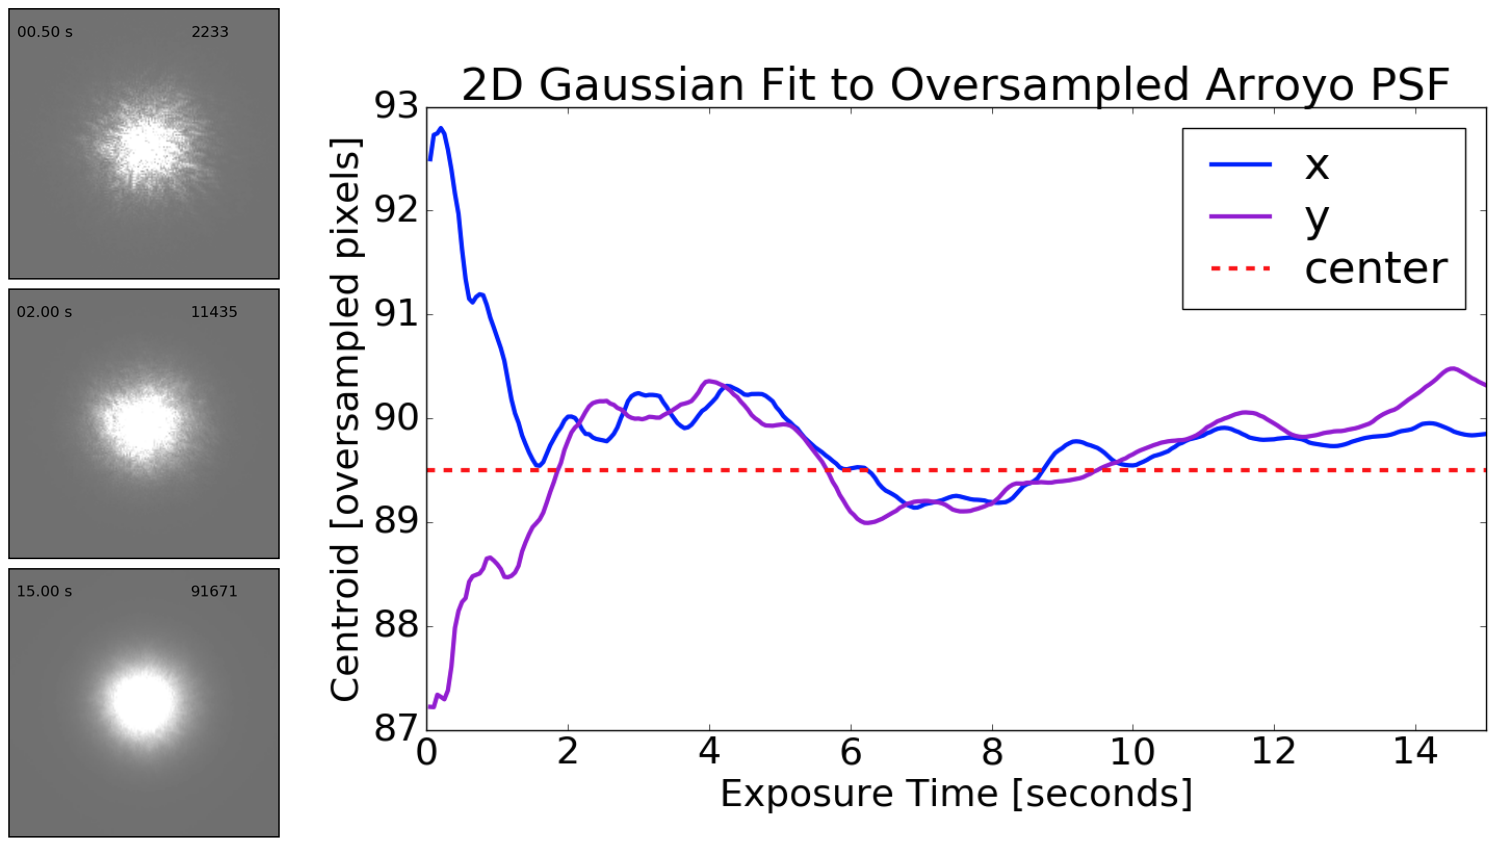
\includegraphics[width=14cm,trim={0cm 0cm 0cm 0cm}, clip]{figures/exptime.png}
\caption{At left, Arroyo atmosphere-only simulated PSF for LSST (with oversampled pixels) with exposure times of 0.5, 2, and 15 seconds (top to bottom), courtesy of Bo Xin. At right, blue and purple lines show the location of the centroid derived from a 2D Gaussian fit to the PSF as a function of exposure time, with the red dashed line showing the true center. We can see that for exposure times greater than 2 seconds, the centroid converges near its true value. \label{fig:expt}}
\end{center}
\end{figure}

(2) Longer Exposures. There is no maximum exposure time specified for an LSST image. Given that the template image will be a stack of at least a year or two of data, processing a $5$--$10$ times deeper single image through the difference imaging pipeline should be fine. However, a $2\times150$ second exposure would saturate at $r \approx 18.3$, and cosmic-ray rejection completeness might suffer (unknown), which could impact the quality of a difference image and the detected sources. With a longer exposure time the $60$ second latency requirement could still be met, but any system qualities that vary on short (but $>30$ second) timescales could inhibit photometric calibration (e.g., tracking). 

In conversation with DM-AP team members (Reiss, Findeisen, Connolly, Bo) there has not yet been a study of the safe range of exposure times that will be allowed to contribute to the Level 1 and Alert Stream. One possibly useful study is Chang et al. (2012), "Atmospheric point spread function interpolation for weak lensing in short exposure imaging data". They show that a 15 second exposure contains PSF variability on short spatial scales across a 1 square degree image which, for extragalactic fields with few stars (i.e., but good for weak lensing), is hard to characterize. They present a new software package to do mitigate the effects. Alternatively, we may need to use software packages {\tt PhoSim} (Peterson et al. 2015; \url{http://adsabs.harvard.edu/abs/2015ApJS..218...14P}) or {\tt ARROYO} (\url{http://proceedings.spiedigitallibrary.org/proceeding.aspx?articleid=848256}) to at least simply characterize the PSF stability as a function of exposure time.


% % % % % % % % % % % % % % % % % % 
\subsection{Summary}\label{ssec:data_summary}

Our review of the technical boundaries and previously proposed Special Programs leads us to conclude that the potential diversity of data is mainly limited to exposures that are significantly shorter than the WFD main survey standard visit exposures of $2\times15$ seconds, and exposures that are obtained with a bright sky background during twilight. 






% % % % % % % % % % % % % % % % % % % % % % % % % % % % % % % % % % % % 
\section{The Current DM Plans for Special Programs Data Processing} \label{sec:dmplans}

As presented in Section \ref{sec:intro}, the intent of LSST DM for processing data from Special Programs can be summarized by the following statement, which reflects Section 6 of the Data Products Definitions Document (DPDD, LSE-163, \cite{LSE-163}):

\begin{quote}
LSST will not write unique algorithms for processing Special Programs data or reprocessing Main Survey data, but LSST will reconfigure the pipelines and generate imaging and catalog products for Special Programs data whenever possible, and LSST will make its codes accessible to the science community and commit $\sim$10\% of its computing resources toward enabling Level 3 analysis and data product creation, including user-driven Special Programs processing.
\end{quote}

In this section we review in greater detail the intent of DM to incorporate Special Programs data into the pipelines and products for the WFD main survey (Section \ref{ssec:dmplans_WFD}), to reconfigure the pipelines and generate unique sets of data products for each Special Program (Section \ref{ssec:dmplans_reconfig}), and to enable Level 3 processing (Section \ref{ssec:dmplans_L3}). Later on, in Section \ref{ssec:dmplans_review}, we review each piece of DM documentation in turn and identify requirements and/or specifications that do not adequately represent the intent of LSST DM, as defined in Section 6 of the DPDD, with respect to Special Programs processing. Where relevant we suggest clarifications, changes, or additions to these documents.

%\begin{enumerate}[topsep=-10pt,label= \textbf{Concern \Roman*.},resume] \item \label{C1} There are currently no requirements on DM to incorporate data from Special Programs; should there be? \end{enumerate}
%\begin{enumerate}[topsep=-10pt,label= \textbf{Concern \Roman*.},resume] \item \label{C2} Should DM undertake an investigation to define the exposure boundaries (integration time, sky background) for non-standard visit images that can be processed by DM pipelines, such as ISR and DIA? \end{enumerate}
%\begin{enumerate}[topsep=-10pt,label= \textbf{Concern \Roman*.},resume] \item \label{C3} Given the double-processing of Special Programs data, is the system sized appropriately? \end{enumerate}


% % % % % % % % % % % % % % % % % % 
\subsection{Intent to Include Special Programs Data in the WFD Survey Products}\label{ssec:dmplans_WFD}

It seems obvious that LSST DM would want to incorporate images obtained through Special Programs into the WFD main survey's pipelines and products whenever it is beneficial for enabling science. In the following three sections we summarize when and how SP data might be incorporated into the pipelines and products of the Level 1 and Alert Stream, the Level 2 DRP, and/or MOPS.

\subsubsection{Level 1 and the Alert Stream}\label{ssec:dmplans_WFD_L1}

It is beneficial to transient science to include as many LSST images into Level 1 and the Alert Stream as possible. Only products of the Level 1 $60$-second processing pipeline can contribute to the Alert Stream: this means that no Level 3 difference imaging pipeline can send its detections to the Alert Stream, although a separate Level 3 alert stream should be possible if the packet/transport mechanism that LSST defines is adopted outside of LSST. Therefore, only images that qualify for Level 1 processing will contribute to the Alert Stream. The template images that are used in the Level 1 difference imaging pipeline will be built from the Level 2 DRP, and so the first factor affecting a SP image's suitability for Level 1 is to be in a region of sky with an existing template. So long as there is a template, when the exposure time is equivalent to a WFD visit image, $\sim 30$ seconds, treating the image as Level 1 is obviously going to be fine. However, the suitability of shorter and longer exposures is unknown, as discussed in Section \ref{ssec:data_DMconstraints}.

\subsubsection{MOPS}\label{ssec:dmplans_WFD_MOPS}

The WFD main survey observations will be optimized to meet the mandated goals for moving object discoveries, so it is unclear whether the science goals of MOPS can be much improved by incorporating Special Programs data. Since MOPS takes {\tt DIASources} as input, any SP images that can be run through the Alert Pipeline can be ingested by MOPS. As discussed under ``Solar System Objects (SSO)" in Section \ref{ssec:data_science}, most of the Special Programs data associated with SSO science will obtain standard visit images anyway.

\subsubsection{Level 2 Data Release Pipeline}\label{ssec:dmplans_WFD_L2}

Unlike with transient detection and the Level 1 Alert Stream, it is not clear whether it is beneficial to the science goals that depend on the Level 2 DRP to include as many LSST images as possible. We propose that the simplest option is probably that LSST DM deliver a single Level 2 DRP {\tt Objects} database that is built from a set of images with nearly constant depth and cadence. When Special Programs data brings additional area up to the same level of depth and cadence as the rest of the WFD main survey, or improves the Level 2 DRP in some other way, it can be included in the Level 2 DRP. For example, photometric calibrations may require that some or all of the (shallower) Galactic Plane Special Program survey area be incorporated in order to suppress edge effects and low-order modes in the photometric solutions. In short, DM should probably not promise to incorporate any specific data into the Level 2 DRP images or catalogs.


% % % % % % % % % % % % % % % % % % 
\subsection{Intent to Process Special Programs Data with Reconfigured DM Pipelines}\label{ssec:dmplans_reconfig}

LSST DM intends to reconfigure its existing pipelines in order to generate imaging and catalog products for Special Programs data, whenever possible. In this context, possible means that no new algorithms need to be written and that an intensive amount of additional computational resources is not required for the processing. In a possible scenario, DM would assemble a pipeline from existing DM codes in order to process data associated with a given Special Program and build unique, separate image and catalog products that meet the science needs of that particular program. For example, for a DDF SN survey (see Section \ref{ssec:SPCS_SNDDF}), existing DM codes would be used to: (1) make a deep template image from a certain time window, (2) process standard single visit images, (3) create a nightly CoAdd, (4) run difference imaging analysis, (5) run source detection on the difference images, and (6) create {\tt DIASource} and {\tt DIAObject} catalog equivalents (this example is also given in Section 6 of the DPDD, \cite{LSE-163}). This type of reconfiguration is also be possible for users to do as a Level 3 pipeline (see below), but having these products provided by DM ensures a consistent and verified level of quality and public access to all processed Special Programs data products, and is expected to be a large benefit to the science results.


% % % % % % % % % % % % % % % % % % 
\subsection{Intent to Support Special Programs Processing with Level 3 Pipelines}\label{ssec:dmplans_L3}

If a Special Program requires processing that cannot be accomplished with existing DM algorithms and codes, and/or requires an intensive amount of additional computational resources, it is considered Level 3 -- and in the latter case the processing might have to be undertaken on a separate computational resource. To support such Level 3 processing DM intends to make the data and its code base accessible to and exportable by users in the science community. In most cases, data export and processing on external computation resources will not be necessary. The majority of users will access the data, build pipelines based on DM codes, and execute them through the Science Platform \cite{LDM-542}. Through the Science Platform, DM provides the infrastructure for users to run their Level 3 pipelines on LSST servers, monitor their progress, and analyze their output. DM will also provide a prioritization system to allocate processing resources in the case of oversubscription. All of this applies to both Level 3 processing for Special Programs data, and reprocessing of WFD main survey data. It is furthermore expected that, over time, some Level 3 pipelines will become "federated", installed and operated (and change controlled) by the LSST Operations team. For both federated and user-run code, whether they are for Special Programs or WFD survey data, the LSST DM team will encourage and facilitate data product databases that are built with the same schema as -- and can easily be joined with -- the tables of Level 1 and 2.

% % % % % % % % % % % % % % % % % %
\subsection{Documentation Review}\label{ssec:dmplans_review}

Here we highlight every requirement or issue relevant to Special Programs that we could find in the existing documentation. Since the goal of this work is to make any needed changes to existing documentation, we have endeavored to directly tie every possible concern to the relevant sections of existing documentation (or, where possible, to requirement codes) so that we can more easily direct future changes back into the existing documentations.


% % % % % % %
\subsubsection{Science Requirements Document, SRD, LPM-17, \cite{LPM-17}}\label{sssec:dmplans_review_srd}

This document does contain requirements for the data that are needed to achieve the main science goals, but the version available at this time is from 7/6/2011, and some specifications are out of date (e.g., the minimum exposure time is set to 5 seconds, in contrast with OSS-REQ-0291). The SRD makes two mentions of Special Programs: that the ``LSST is well suited to conducting Deep Supernova Survey" (Section 2.3), and that 90\% of the observing time will be spent on the main survey, with the remaining 10\% used for a variety of other programs (Section 3.4). The latter we know to be an approximate estimate.


% % % % % % %
\subsubsection{LSST System Requirements, LSR, LSE-29, \cite{LSE-29}}\label{sssec:dmplans_review_lsr}

The LSR is derived from the SRD, and converts the high-level specifications from the SRD into system requirements, which flow-down to and in some cases repeated in the OSS and DMSR (next sections). We have the version of LSE-29 last revised on August 4, 2016.

\begin{enumerate}[topsep=-10pt,after=\vspace{10pt},label= \textbf{Concern \Roman*.},resume] \item \label{LSR-0} Most notably, there is no written requirement for DM to reconfigure its pipelines and produce unique, separate data products for the accepted Special Programs, wherever possible, as it intends to. Should there be, and is the LSR right right place for it? \end{enumerate}

\begin{enumerate}[topsep=-10pt,after=\vspace{10pt},label= \textbf{Concern \Roman*.},resume] \item \label{LSR-0b} Similar to \ref{LSR-0}, there is no written requirement for DM to evaluate the benefit of incorporating data from Special Programs into the products of the WFD main survey, and then to do this when it is found to enable/improve science results, as it intends to. Should there be, and is the LSR right right place for it? \end{enumerate}

$\bullet$ LSR-REQ-0102 defines the minimum interval between data releases to be {\tt DRT1} = 1 year (1.4.2, Data Release Processing).
\begin{enumerate}[topsep=-10pt,after=\vspace{10pt},label= \textbf{Concern \Roman*.},resume] \item \label{LSR-1} There is no requirement on the schedule or latency for delivering Special Programs data products that is equivalent to the requirements for delivery of yearly data releases (LSR-REQ-0102; LSE-29). Should there be? \end{enumerate}

$\bullet$ LSR-REQ-0111 requires that LSST be capable of obtaining \textit{and processing} exposures that were not taken in a standard visit mode, including those with minimum exposure time of {\tt minExpTime} = 1 second, with the caveat that ``non-standard visit exposures may possibly be degraded in some aspects of performance (e.g., cosmic ray rejection)" (2.3.1.2, Non-Standard Visit).
\begin{enumerate}[topsep=-10pt,after=\vspace{10pt},label= \textbf{Concern \Roman*.},resume] \item \label{LSR-2} While the requirement that LSST process non-standard visit exposures (LSR-REQ-0111, LSE-29) implies that DM must be able to process the full diversity of Special Programs data, it should probably be verified that this is (a) true and (b) possible. For example, will DM impose limitations on the exposure times for which the Instrument Signature Removal (ISR) processing can deliver a science-grade quality image, as considered in Section \ref{ssec:data_DMconstraints}? \end{enumerate}

$\bullet$ LSR-REQ-0032 requires that the LSST DM system provide three classes of science data products as ``Level 1 (nightly cadence), Level 2 (data release cadence), and Level 3 (user-specified)", and subsequent sections describe the products and their timescales for delivery (2.4.5.1 Organization of Data Products).
\begin{enumerate}[topsep=-10pt,after=\vspace{10pt},label= \textbf{Concern \Roman*.},resume] \item \label{LSR-3} It might be helpful to include in this section that Special Programs processing with reconfigured Level 1 and 2 codes, wherever possible, is also an effective requirement similar to LSR-REQ-0032 (LSE-29). (This might satisfy \ref{LSR-0}). \end{enumerate}

$\bullet$ LSR-REQ-0041 requires that LSST support Level 3 data products ``of a nature specified by users", and LSR-REQ-0106 that LSST provide software, services, and hardware resources to enable the production and storage of those products (2.4.5.1, Organization of Data Products).
\begin{enumerate}[topsep=-10pt,after=\vspace{10pt},label= \textbf{Concern \Roman*.},resume] \item \label{LSR-4} The requirements for LSST to provide software, services, and hardware resources to support Level 3 data products (LSR-REQ-0041, LSE-39) all have technical limits (i.e., DM's intent to create and run reconfigured pipelines for Special Programs data ``unless it requires an intensive amount of additional computational resources" as discussed in Section \ref{ssec:dmplans_L3}); should these be mentioned in the LSR? (Or are they just in the sizing documents, discussed in Section \ref{sssec:dmplans_review_sizing}?)  \end{enumerate}

$\bullet$ LSR-REQ-0042 requires that LSST produce the data products necessary to support the four primary science missions (dark energy, solar system, transients, milky way; 2.4.5.2, Science Flowdown). 
\begin{enumerate}[topsep=-10pt,after=\vspace{10pt},label= \textbf{Concern \Roman*.},resume] \item \label{LSR-5} The requirement for LSST to produce the data products necessary for the four primary science missions (LSR-REQ-0042, LSE-29) could be extended with text to include Special Programs data? This is might also satisfy \ref{LSR-0}. \end{enumerate}

$\bullet$ LSR-REQ-0055 requires that {\tt userComputingFraction} = 10\% of the total LSST data processing capacity and storage space be allocated for user analysis and Level 3 pipelines and products (2.5.6, Community Computing Services). This is discussed further in Section \ref{sssec:dmplans_review_sizing}.

$\bullet$ LSR-REQ-0075 defines that the WFD main survey science objectives will be met with 90\% of the observing time, with the remainder left to Special Programs (Section 3.3.1, Survey Time Allocation) 


% % % % % % %
\subsubsection{Observatory System Specifications, OSS, LSE-30, \cite{LSE-30}}\label{sssec:dmplans_review_oss}

The OSS contains the requirements on the site, facility, and camera that are necessary to meet the requirements specified by the LSR (LSE-29) and the SRD (LPM-17). We have the version of LSE-30 last revised on February 10, 2017. For the most part, the {\bf Concerns} raised in this section are not relevant to Data Management and are probably outside the scope of this study. But we keep them because they are relevant to Section \ref{ssec:data_bounds}. 

$\bullet$ OSS-REQ-0027 requires that the scheduling system be able to optimize over at least {\tt nSciProp} = 6 ``science proposals", where these ``proposals" are observing targets/constraints such as the distribution of filters, the astronomical conditions, and relative priority (2.1.1.2, Multiple Science Programs). 
\begin{enumerate}[topsep=-10pt,after=\vspace{10pt},label= \textbf{Concern \Roman*.},resume] \item \label{OSS-1} There is a requirement on the minimum number of ``science proposals" that can be optimized by the scheduler ({\tt nSciProp} = 6, OSS-REQ-0027, LSE-30), but is there also a technical constraint on the maximum? This might be relevant to some proposed mini-surveys with complicated observing strategies. \end{enumerate}

$\bullet$ OSS-REQ-0381 requires that the schedule be able to handle targets of opportunity, which would be relevant for e.g., Special Programs for gravitational wave follow-up (2.1.1.7, Visit Optimization).

$\bullet$ OSS-REQ-0189 and OSS-REQ-0190 set the minimum number of raw exposures to be supported as {\tt nRawExpNightWinterAvg} = 1960 per night on average (but up to {\tt nRawExpNightMax} = 2800 per night if e.g., two hours of a short-exposure twilight mini-survey are included) and {\tt nRawExpYear} = 5.5$\times10^5$ per year, respectively. These numbers are set by predicting the maximum number of exposures that would be acquired on the longest night of the year in WFD cadence with 2 second slews, assuming $\sim80\%$ completion, but adding a 10\% margin. These estimates appear adequate for Special Programs in general.

$\bullet$ OSS-REQ-0194 and OSS-REQ-0323 set the minimum number of calibration exposures to be supported as {\tt nCalibExpDay} = 450 per night on average and {\tt nCalExpYear} = 1.5$\times10^5$ per year, respectively. 
\begin{enumerate}[topsep=-10pt,after=\vspace{10pt},label= \textbf{Concern \Roman*.},resume] \item \label{OSS-2} There is a requirement on the minimum number of calibration frames that will be supported during daytime ({\tt nCalibExpDay} = 450, OSS-REQ-0194, LSE-30); could we imagine a Special Program that would need more than that? \end{enumerate}

$\bullet$ OSS-REQ-0125, Section 3.1.5 deals with data products, including requirements for the variety and format of data products (i.e., images and catalogs in Level 1 and 2), the precision of the data products (e.g., photometric and astrometric accuracy, completeness/spurious thresholds for DIA sources), and the timeline for the release of data products (alerts, Level 1, and the Level 2 DRP).  (Section 3.1.5, Data Products).
\begin{enumerate}[topsep=-10pt,after=\vspace{10pt},label= \textbf{Concern \Roman*.},resume] \item \label{OSS-3} There are requirements on the type and quality of data products for Level 1, 2, and 3 (OSS-REQ-0125 and all those following, in LSE-30). Should it be specified, for Special Programs data, whether or which of these requirements DM must meet? For example, OSS-REQ-0157 sets the fraction of false detections in deep CoAdds caused by unremoved artifacts to be {\tt falseDeepDetect} = 0.1\%, but would this apply to a DDF stack? \end{enumerate}

$\bullet$ Section 3.5, Photometric Calibration, puts requirements on e.g., the relative contributions to photometric errors from instrumental (OSS-REQ-0282) and atmospheric (OSS-REQ-0276) transmissions, and that a catalog of$10000$ reference stars of $17<r<20$ mag per field be created for use (OSS-REQ-0285). It seems that these might not apply to non-standard images from Special Programs (3.5, Photometric Calibration).
\begin{enumerate}[topsep=-10pt,after=\vspace{10pt},label= \textbf{Concern \Roman*.},resume] \item \label{OSS-4} Section 3.5 of the OSS (LSE-30) puts requirements on the photometric calibrations for WFD data, but it is unclear how and whether these requirements extend to DM providing calibration of non-standard images from Special Programs (this is related to \ref{LSR-2}). \end{enumerate}

$\bullet$ OSS-REQ-0319 sets the requirement that the LSST be capable of continuous operation throughout the night when all visits are separated only by the readout time, thereby enabling a deep drilling field style of observations (3.6.1.3, Continuous Exposures).

$\bullet$ OSS-REQ-0291 defines the minimum exposure time as $1$ second with a stretch goal of $0.1$ seconds, with a note that the spacing between exposures may need to be lengthened in order to maintain camera thermal stability, and that the thermal stability might also be affected with longer exposure times (3.6.1.4, Minimum Exposure Time). \\
\begin{enumerate}[topsep=-10pt,after=\vspace{10pt},label= \textbf{Concern \Roman*.},resume] \item \label{OSS-5} There is a requirement on the minimum exposure time (OSS-REQ-0291, LSE-30), but not on the spacing between short exposures and no specified maximum exposure time. It would be great to get this clarified from the camera team and updated in the OSS, so we know if they will they impose boundaries on Special Programs data. \end{enumerate}

$\bullet$ OSS-REQ-0293 requires that the maximum time for an operational filter change be {\tt tFilterChange} = 120 seconds (unlikely to be much lower in practice), and OSS-REQ-0295 requires that the LSST support at least 4 changes per night (and 8 in the day). There is no officially required minimum time between filter changes. Unofficially, this is constrained by the total lifetime number of filter changes is $100,000$ over $15$ years, or an average of $18$ changes per night\footnote{From Zeljko.}. Additionally, changes regarding the requirements on filters in support of ``deep drilling fields" are underway here: \url{https://project.lsst.org/groups/ccb/node/938}. (3.6.2 Filter Swaps \& Changes).
\begin{enumerate}[topsep=-10pt,after=\vspace{10pt},label= \textbf{Concern \Roman*.},resume] \item \label{OSS-6}   There are currently are no official requirements on the minimum time between filter changes, only that the time for a filter change will be 120 seconds (OSS-REQ-0293). Should the OSS include a clarification that there is no technical constraint on the frequency of filter changes? ({\it MLG -- maybe unnecessary.}) \end{enumerate}

$\bullet$ OSS-REQ-0301 and OSS-REQ-0300 set the minimum time for continuous rotation tracking ({\tt rotTrackTime} = 1 hour) and the half-range of the rotator motion ({\tt rotTrackRange} = 90 minutes) respectively, but there do not seem to be any constraints on the speed of the rotator or the minimum distance between successive visits (3.6.3.2, Field de-rotation). 
\begin{enumerate}[topsep=-10pt,after=\vspace{10pt},label= \textbf{Concern \Roman*.},resume] \item \label{OSS-7} The OSS contains requirements for rotator capability (OSS-REQ-0301, -0300), but is there a maximum rotation speed, or a limit on the amount of rotation per night (or in a 10-year lifetime), that might constrain the distance between successive visits or the ability to jump between two widely separated fields? \end{enumerate}

$\bullet$ OSS-REQ-0380 sets the rate and error limits for nonsidereal tracking, which presumably would only be relevant to a Special Program (3.6.3.7, Non-Sidereal Tracking).


% % % % % % %
\subsubsection{Data Management Subsystems Requirements, DMSR, LSE-61, \cite{LSE-61}}\label{sssec:dmplans_review_dmsr}

The DMSR contains the top-level requirements for all of Data Management, including processing pipelines and products (revision 2017-08-11).

$\bullet$ DMS-REQ-0068 requires that each raw science image store metadata regarding the date/time, site, telescope, and camera -- missing from this is the scheduler and program information? That kind of metadata will be necessary to identify images related to Special Programs (1.2.3, Raw Science Image Metadata). Related to this is DMS-REQ-0266, which requires the creation of an Exposure Catalog that also stores this kind of metadata independently, but also does not include scheduler and program information. 
\begin{enumerate}[topsep=-10pt,after=\vspace{10pt},label= \textbf{Concern \Roman*.},resume] \item \label{DMSR-1} Clarify if and how scheduler and program information (i.e., identification of an image as being associated with a Special Program) is included in the raw science image metadata and/or the Exposure Catalog (DMS-REQ-0068, -0266); if not, should it be added? \end{enumerate}

$\bullet$ DMS-REQ-0069 requires that DM produce processed visit images (overscan trimmed, ISR, snap-combined), and that they are not archived (but can be regenerated on demand). It also says that ``this aspect of the processing for Special Programs data is specific to each program". It should be specified whether ``this aspect" refers to the reduction or archiving of the processed visit images; if processed visit images for Special Programs can live on disk for longer, does this affect the sizing models? (1.2.2, Processed Visit Images). This question applies also to DMS-REQ-0010, which requires that DM create one difference image for each processed visit image (1.3.3, Difference Exposures).
\begin{enumerate}[topsep=-10pt,after=\vspace{10pt},label= \textbf{Concern \Roman*.},resume] \item \label{DMSR-2} Confirm whether processed single visits and/or difference images for Special Programs can stay on disk and accessible to e.g., Level 3 pipelines, for a longer amount of time by user request (DMS-REQ-0069 and -0010, LSE-61). \end{enumerate}

$\bullet$ DMS-REQ-0069 and DMS-REQ-0010 require that DM create processed single visit images and a difference image for each of those, but this might not be possible for Special Programs that obtain non-standard exposures (i.e., short exposures in which the PSF is not well formed, or very bright sky backgrounds). 
\begin{enumerate}[topsep=-10pt,after=\vspace{10pt},label= \textbf{Concern \Roman*.},resume] \item \label{DMSR-3} Confirm the exposure boundaries for which DM can produce processed single visits and/or difference images for Special Programs that obtain non-standard images (DMS-REQ-0069 and -0010, LSE-61). This is related to \ref{LSR-2} and might require a dedicated additional study with simulated data, as discussed in Section \ref{ssec:data_DMconstraints}. \end{enumerate}

$\bullet$ DMS-REQ-0274 sets the content of an Alert, but this does not currently include scheduler or program information; should this be added? This would enable users to e.g., use the LSST mini-broker to filter for only Alerts from their desired Special Program, in case they have a dedicated follow-up resource. Furthermore, it might facilitate follow-up more generally if users know e.g., that this Alert is from a field that is going to be observed again in $X$ minutes or $Y$ times in a night (1.3.13, Alert Content). However, the latter might be adequately available through the predicted visit schedule server specified by DMS-REQ-0353.
\begin{enumerate}[topsep=-10pt,after=\vspace{10pt},label= \textbf{Concern \Roman*.},resume] \item \label{DMSR-4} Could and/or should we add the program information and/or predicted revisit schedule to the Alert content (if it isn't included already)? (DMS-REQ-0274, -0353) \end{enumerate}

$\bullet$ DMS-REQ-0320 states that ``it shall be possible for special programs to trigger their own data processing recipes", but this could use clarification. It could be misinterpreted to mean that the {\it science users} must trigger the processing, thereby classifying it as Level 3. More likely, it means that e.g., a header keyword identifying an image as related to a Special Program is sufficient to send it to a dedicated processing pipeline. (1.6.1 Processing of Data From Special Programs)
\begin{enumerate}[topsep=-10pt,after=\vspace{10pt},label= \textbf{Concern \Roman*.},resume] \item \label{DMSR-5} Can we clarify the mechanism by which Special Programs trigger their own data processing recipes, as required by DMS-REQ-0320? \end{enumerate}

$\bullet$ DMS-REQ-0321 and DMS-REQ-0344 together specify that the Level 1 processing from Special Programs shall be completed with the same latencies as applied to data from the WFD main survey. It should probably be specified that this applies only to Special Programs data that consists of standard visit images (and not, e.g., very short or very long exposure times unless they can be shown to result in quality difference images), and that ``reporting optical transients" within {\tt OTT1} = 1 minute means contributing to the L1 Alert Stream. (1.6.2 Level 1 Processing of Special Programs Data, 1.6.3 Constraints on Level 1 Special Program Products Generation)
\begin{enumerate}[topsep=-10pt,after=\vspace{10pt},label= \textbf{Concern \Roman*.},resume] \item \label{DMSR-6} Clarify that only Special Programs data that {\it can} be incorporated into the Level 1 pipeline (i.e., standard visit images, or non-standard visit images that can be shown to result in quality DIA products; see \ref{DMSR-3}), will be incorporated (relevant also to \ref{LSR-0b}, \ref{LSR-2}). Perhaps add that in these cases they will contribute directly to the L1 Alert Stream, with a note that generating a separate Level 3 stream of alerts specific to a Special Program should also be possible (DMS-REQ-0321, -0344). \end{enumerate}

\begin{enumerate}[topsep=-10pt,after=\vspace{10pt},label= \textbf{Concern \Roman*.},resume] \item \label{DMSR-6b} Related to \ref{DMSR-6} and DMS-REQ-0344, there is also a potential problem with short exposures (e.g., 5 seconds) that can be processed by  the DIA pipeline, but pose a problem for the Alert Stream because the higher data acquisition rate (e.g., $\sim$6$\times$ higher) would cause a processing back-up. Should this situation arise, are there options for short-term increases in parallel processing power at NCSA? Such options might also apply to e.g., crowded fields with $>$10k {\tt DIASources}. \end{enumerate}

$\bullet$ DMS-REQ-0322 specifies that data products from Special Programs processing shall be stored in separate (but joinable) databases.

Section 1.6 ``Special Programs" might benefit from the addition of discussion and/or requirements to address the following: \\
$\bullet$ Should we add a general specification to the DMSR (\S~1.6) to describe whether and how data from Special Programs could be included in the WFD main survey Level 1 and/or 2 data products, as also raised for the LSR in \ref{LSR-0b}, and as discussed in Section \ref{ssec:dmplans_WFD}? \\
$\bullet$ Should we add a specification to the DMSR (\S~1.6) to describe DM's plans to reconfigure its own pipelines for the processing of Special Programs data, perform and verify this processing, and deliver the unique products (separate but joinable to the WFD L1 and L2 products), as also raised for the LSR in \ref{LSR-0}, and as discussed in Section \ref{ssec:dmplans_reconfig}? \\
$\bullet$ Since DM plans to include Special Programs data to the WFD main survey's L1 and L2 products wherever possible, and also run dedicated processing and generate unique products for all SP data, the associated computational and storage resources for Special Programs data might need to be multiplied by {\it at least} a factor of two. This is discussed more in Section \ref{sssec:dmplans_review_sizing}, but should it also be addressed in the DMSR?

$\bullet$ The following items are applicable to users processing data from Special Programs and/or reprocessing data from the WFD main survey. Since they're relevant to Special Programs, we mention them here, but they have not spawned any concerns. Section 2.9 ``Level 3 Production" includes the requirements on access controls, external data, processing resource prioritization, consistency, provenance, and providing a software framework. Sections 3.1 ``Software Architecture to Enable Community Re-Use" and 3.2 ``Applications Software" describe aspects of the DM system that will be important to users, such as that the codes be extendable to both high-performance and desktop platforms, be able to handle simulated data and data from other instruments, and that a user interface will be provided. In Section 3.3 ``Middleware Software", DMS-REQ-0298 requires that DM provide software to list and retrieve data, including raw data (3.3.2.2, Data Product and Raw Data Access), along with other user-access issues.

$\bullet$ DMS-REQ-0312 and -0313 require that DM maintain a live L1 and the two most recent DR L1 and L2 catalogs for access by users, but there is no corresponding access requirement for the data products of Special Programs (4.1, Data Archive).
\begin{enumerate}[topsep=-10pt,after=\vspace{10pt},label= \textbf{Concern \Roman*.},resume] \item \label{DMSR-10} Should there be a requirement for maintenance of user access to data products of Special Programs with the same timescales as the WFD main survey data, similar to DMS-REQ-0312, -0313? (This is related to \ref{LSR-1}) \end{enumerate}


% % % % % % %
\subsubsection{Data Management Applications Design, DMAD, LDM-151, \cite{LDM-151}}\label{sssec:dmplans_review_dmad}

The DMAD specifies the design and implementation of the code and algorithms that will be used in the processing of images and creation of catalogs in the Level 1 AP, Level 2 DRP, and MOPS pipelines. We have used the version last revised 2017-07-19. As the DMAD focuses on the content of the code and algorithms, it is relatively agnostic as to whether the source of the data is the WFD main survey or Special Programs -- but does (in some places) explicitly assume standard visit images of $2\times15$ seconds as the raw image input. In fact, the phrase ``Special Programs" appears four times: three times as a source of reference catalogs or training sets, and once as a potential source of visits that have only a single $15$ second snap. It is the DMAD's codes and algorithms that DM will be {\it reconfiguring} to create pipelines for Special Programs -- any new algorithms that might enable science from Special Programs are considered beyond the scope of DM and will need to be developed as Level 3. This document will be handy to use in conjunction with Special Programs processing case studies (e.g., Section \ref{sec:SPCS}) that will be included with the next call for white paper proposals (Section \ref{ssec:data_comm}). 

The purpose of this study on Special Programs is not to suggest any changes to the DMAD. Instead, here we list a couple of examples of algorithms that sit at the threshold between DM-produced and Level 3: {\bf Deblending --} The deep deblender algorithm described in Section 5.3.3 will, out of necessity, be optimized for use in the bulk of the WFD main survey. It may or may not end up being appropriate for use in the Galactic Plane mini-survey area, depending on the science goal. Level 3 deblenders for specific Special Programs fields may require development by the user community. {\bf Variability Characterization --} The periodic and aperiodic variability characterizations described in Section 6.21 are placeholders, but are representative of what is likely to be implemented: algorithms that are applicable to a broad range of variability types. From DM's perspective, all that is needed is sufficient information to enable relatively useful filters, from which the downstream broker/user can do additional filtering, and these parameterizations might not be sufficient for all science goals. It is conceivable that the goals of a particular Special Program might require different algorithms, and these would be written as Level 3 and either made joinable to the DM reconfigured data products, or perhaps federated and incorporated directly. {\bf Photometric Redshifts --} As described in Section 5.6.5 the Level 2 DRP {\tt Object} catalog will include a photometric redshift, but this algorithm will be produced by the science community and then federated and run at scale by DM. It is conceivable that the photo-$z$ algorithm for a Special Programs data set product might be different from that used for the WFD main survey. 


% % % % % % %
\subsubsection{Data Products Definitions Document, DPDD, LSE-163, \cite{LSE-163}}\label{sssec:dmplans_review_dpdd}

The DPDD describes the data products -- the images and catalogs -- to be delivered from the Level 1 AP, Level 2 DRP, and MOPS pipelines. We have used the version last revised 2017-07-01. Section 6 describes the data products that DM will provide for Special Programs. It specifies that the processing will use the same software stack as the Level 1 and 2, will make separate imaging products and separate (but joinable) catalogs, and use $\lesssim10\%$ of the computational and storage facility of the total LSST processing cluster (see Section \ref{sssec:dmplans_review_sizing} for sizing questions). 

The LSST Database Schema Browser\footnote{\url{http://lsst-web.ncsa.illinois.edu/schema/index.php?sVer=baseline}} is another way to explore the contents of the planned DM catalogs. We identify a couple of potential changes that might be necessary to the schema, which are related to this study on Special Programs. These are not high priority.

$\bullet$ The database schema for {\tt DIASource} does not appear to have an element that identifies which template image that was used. This will be needed for both Levels 1 and 3 differencing pipelines and products, for both Special Programs and WFD main survey data. DMS-REQ-0074 already does require that the identity of input exposures is stored for each difference image (LSE-61).
\begin{enumerate}[resume,topsep=-10pt,label= \textbf{Concern \Roman*.}] \item \label{C8} Database schema for {\tt DIASource} might need to have an element added that contains information about the template that was used to create the difference image, unless it can be shown that this can be handled by provenance (i.e., the code version and time of processing are sufficient to deduce which template was used). \end{enumerate}

$\bullet$ The DMAD specifies that externally defined targets can be incorporated into the {\tt Objects} catalog (Section 3.2.5), and this may be a particular interest to Special Programs. It is unclear how such targets will be identified or flagged as such in the database schema, and whether we need to add an element for this. Currently, the {\tt Object} database contains an element {\tt prv\_inputId} which is an {\tt integer}, and is described as the {\it ``Pointer to prv\_InputType. Indicates which input was used to produce a given object."} Is that all we need? \\
\begin{enumerate}[resume,topsep=-10pt,label= \textbf{Concern \Roman*.}] \item \label{C9} Clarify whether {\tt Object.prv\_inputID} will identify whether an {\tt Object} is an externally provided coordinate. \end{enumerate}

$\bullet$ As described in the DMAD and the DPDD, these are the {\tt Object} and {\tt DIAObject} elements that have been reserved for variability characterization: \\
{\tt Object} and {\tt DIAObject.lcPeriodic} = {\tt float[6 x 32]} = Periodic features extracted from light-curves using generalized Lomb-Scargle periodogram \\
{\tt Object} and {\tt DIAObject.lcNonPeriodic} = {\tt float[6 x 32]} = Non-periodic features extracted from light-curves using generalized Lomb-Scargle periodogram \\
Section 6.21 of the DMAD describes the nominal algorithms to define these parameters, but as we mentioned in Section \ref{sssec:dmplans_review_dmad}, different kinds of variability might be measurable Special Programs cadences that are quite different from the WFD main survey. Are 32 floats in each of the 6 filters always going to be a large enough volume? ({\it MLG -- I suspect yes and that if not, compression can be used, but am leaving this note here anyway}).
\begin{enumerate}[resume,topsep=-10pt,label= \textbf{Concern \Roman*.}] \item \label{C10} DM might want to consider whether {\tt float[6x32]} for the characterization parameters for variability is adequate to express the additional timescales and depths covered by all possible Special Programs observing strategies. This might be similar to e.g., DMTN-049 for photometric redshifts included in the Level 2 DRP {\tt Object} catalog. \end{enumerate}


% % % % % % %
\subsubsection{Photometric Calibration for the LSST Survey, LSE-180, \cite{LSE-180}}

LSE-180 is built on {\tt OpSim} runs that do include some nominal DDF, but the photometric calibration investigated in this work does not much deal with potential issues induced by non-standard visit patterns or exposure times of Special Programs, as its scope is the WFD main survey. Potential issues with DM processing -- including calibrations -- of non-standard visit exposure times is raised in Section \ref{ssec:data_DMconstraints} and \ref{LSR-2}. Regarding the reduction and calibration of non-standard visit imags, LSE-180 makes two relevant points: \\
$\bullet$ In LSE-180, it is assumed that all factors affecting the system transmission are stable on 15 second timescales (page 10), but not what the upper limit of that might be. \\
$\bullet$ LSE-180 comments on the dither pattern for the WFD survey in that "dither patterns where the overlap is one quarter of the field of view or more produce results meeting the SRD requirements", but this is specific to photometric calibration of the WFD. The LSE-180 also mentions that an inappropriate dither pattern can make it hard to correct for the variation of system bandpass as a function of the focal plane position -- but so long as this is solved in the WFD, the corrections can be applied to the much smaller amount of data from the Special Programs.


% % % % % % %
\subsubsection{Computational Resources Sizing Documentation}\label{sssec:dmplans_review_sizing}

LSST Science and Project Sizing Inputs spreadsheet (LSE-81) and explanation document (LSE-82) states that 10\% of the computing and storage resources estimated as necessary for the completion of the WFD Main Survey has been added to accommodate Level 3 data products. DM Compute Sizing spreadsheet (LDM-138) and explanation document (LDM-140) estimates the total compute resources needed for all processes, quoting the same 10\% addition for Level 3. DM Storage and I/O Sizing spreadsheet (LDM-141) and explanation document (LDM-139) estimates the total hardware needs, quoting the same 10\% addition for Level 3. As mentioned in Section \ref{sssec:dmplans_review_lsr}, LSR-REQ-0055 requires that {\tt userComputingFraction} = 10\% of the total LSST data processing capacity and storage space be allocated for user analysis and Level 3 pipelines and products. In Section 6 of the DPDD, it is specified that the DM-provided processing of data from Special Programs will ``use no more than $\lesssim10\%$ of computational and storage capacity of the LSST data processing cluster". The following might be specified in one of the sizing documents, but I am still confused:
\begin{enumerate}[topsep=-10pt,after=\vspace{10pt},label= \textbf{Concern \Roman*.},resume] \item \label{CS-1} Are there two {\it separate} blocks of ``10\% of the computing resources" allocated for DM processing of Special Programs data {\it and} end-user Level 3 analysis, or are these needs coming from the {\it same} 10\%? \end{enumerate}

Most Special Programs data will generate double the amount of processing and products: first, if and when they are incorporated into L1 and L2, and second, when their DM-provided reconfigured pipelines are run to generate independent and unique deep co-adds and catalogs. The Special Programs data also seems more likely than the WFD data to be processed a third time as part of science users Level 3 pipelines. 
\begin{enumerate}[topsep=-10pt,after=\vspace{10pt},label= \textbf{Concern \Roman*.},resume] \item \label{CS-2} Is ``10\% of the computing resources" allocated for DM processing of Special Programs data adequate, or too small, given that it is most likely to be multiply-reprocessed? \end{enumerate}

Regarding the possibly computationally intensive (e.g., shift-and-stack) but scientifically necessary processing that will be done for Special Programs data, it is unclear whether the location for this has been identified; Mario asks {\it "whether this the same batch system we make available to the users for running Level 3 codes or the one that's used to process calibrations. Have these systems been sized?"}.
\begin{enumerate}[topsep=-10pt,after=\vspace{10pt},label= \textbf{Concern \Roman*.},resume] \item \label{CS-3} Confirm on which batch system the bulk of the intensive Level 3 processing -- for Special Programs or WFD main survey -- will take place. \end{enumerate}



% % % % % % %
\subsection{The Limited Documentation Regarding Image Detection Efficiencies}

Characterizing the detection efficiencies will be just as important to Special Programs data as the Wide-Fast-Deep survey. Options such as planting fake sources may be both more manageable and more important to some Special Programs science goals. What, exactly, are the requirements on DM to provide detection efficiencies, and what are the current plans for providing this? Note that here we are talking about planting fakes in the single images for transient detection efficiencies with difference imaging analysis, and not planting fakes in the CoAdds for point-source limiting magnitudes).

$\bullet$ The DPDD (LSE-163) does not have any specific data product related to detection efficiencies, but Section 3.2 "Image Characterization Data" does specify that {\it "Each processed image .. will record information on the pixel variance ... as well as the per-pixel masks ... These will allow the users to determine the validity and usefullness of each pixel in estimating the flux density recorded in that area of the sky"}.

$\bullet$ The DMSR (LSE-61), Section 1.2.11 "Level 1 Data Quality Report Definition" (ID: DMS-REQ-0097): {\it "The DMS shall produce a Level 1 Data Quality Report that contains indicators of data quality that result from running the DMS pipelines, including at least ... detection efficiency for point sources vs. mag for each utilized filter."} However, this is a nightly data quality assessment and not a per-image product. 

$\bullet$ The DMAD (LDM-151), Section 5.6.3 "MakeSelectionMaps", states that this calibration step {\it "is responsible for producing multi-scale maps that describe LSST's depth and efficiency at detecting different classes of object. The details of what metrics will be mapped, the format and scale of the maps (e.g. hierarchical pixelizations vs. polygons), and the way the metrics will be computed are all unknown"}. It also states that this must be extendable to Level 3, but that {\it "the details of what DM will provide still needs to be clarified to the community"}, and notes that the reprocessing time for fake plants could be prohibitive. (Section 3 "Alert Production" also specifies that in LDM-151 {\it "we do not address estimation of the selection function for alert generation through the injection of simulated sources ... Source detection thresholds can be estimated through the use of sky sources"}.)

$\bullet$ Suchyta et al. (2016) presents {\tt balrog}, a fake-embedding software package for detection efficiencies, and applies it in demonstration to DES data (it's not just for point sources, but uses {\tt galsim} to embed shapes built of e.g., Sersic profiles).

$\bullet$ In a UW DM Brown Bag lunch meeting, it became clear that while there are many opinions on how to plant fake sources, not only are there no actual plans to do this, but there is no funding or FTQs allotted to figure out how the deliverable of detection efficiencies should be achieved.

$\bullet \bullet \bullet$ {\bf Summary.} {\it MLG - Perhaps I could take this on as a future study, and assess our options, their costs, and the scientific payoff. Since this is not a question limited to DM processing of Special Programs data, specifically, I end this side note here and no {\bf Concerns} are spawned.}






% % % % % % % % % % % % % % % % % % % % % % % % % % % % % % % % % % % % 
\section{Special Programs Processing Case Studies}\label{sec:SPCS}

For further insight to the DM-related needs of potential Special Programs, we can write out all of the data acquisition and processing steps, in order, that some of the proposed Special Programs might use. This kind of thought experiment of describing the reductions and processing could also be a required section of all future white paper proposals. Note that we are not including any analysis in these descriptions. Also, they aren't that fully realized yet, and could use some more thought and input.

Generic steps currently include: \\
Step 1. Data Acquisition. \\
Step 2. Inclusion in Level 1 AP. \\
Step 3. Delivery of LSST Processed Images. \\
Step 4. Level 3 Processing. \\
Step 5. Level 3 Products. \\
(Step 6. Inclusion in Level 2.) \\

\subsection{A Mini-Survey Searching for TNOs with Shift-and-Stack}\label{ssec:SPCS_MM}

This Special Programs processing summary is based on Becker et al. (2011) white paper to find TNOs with shift-and stack \citep{BeckerWP}. {\it MLG: See Section \ref{sssec:science_dmsums_generic} for a more general processing case-study written by Mario, for a shift-and-stack Level 3 pipeline running regularly on a large amount of data.}

Step 1. Data Acquisition. \\ The observational sequence is triggered. In a single night, the 9 adjacent fields in a 3x3 grid are observed with $336$ $\times$ $15$ second $r$-band exposures. This sequence is always repeated 2-3 nights later. This re-visit sequence is repeated 3 more times: 1.5 months, 3 months, and 13.5 months later. Data obtained in the $g$-band filter is also acceptable. \citep{BeckerWP}

Step 2. Inclusion in Level 1 AP. \\ Each $2\times15$ second visit is processed as Level 1 and Alerts are released within 60 seconds.

Step 3. Delivery of LSST Processed Images. \\ The raw, reduced, and calibrated exposures and difference images from the Level 1 pipeline are made available within {\tt \textbf{L1PublicT}} (currently 24 hours, but see Section \ref{ssec:dmplans_reconfig}). However, this Special Program appears to require a year of dispersed observations before the Level 3 processing would run.
\begin{enumerate}[resume,topsep=-10pt,label= \textbf{Concern \Roman*.}] \item \label{C13} Will there be a Science Platform capability set up so that users are notified not just when any data for their Special Program is taken, but when certain sets are finished and ready for processing? \end{enumerate}

Step 4. Level 3 Processing. \\ The Level 3 pipeline running the shift-and-stack processing will be set up and submitted for batch processing by the user through the Science Platform (this particular Special Program does not appear to need regular or urgent processing, and so its Level 3 code will probably not be federated). Pipeline inputs will be the 336 processed exposures per field per re-visit sequence. The Level 2 difference imaging routine will be used with the same template tract/patch for all. Custom code will shift the difference images, then Level 2 routines will stack and do source detection and characterization (including real/bogus?) and generate an object database. Custom code will derive orbital parameters for the detections and add them to the database. The user is notified with processing status updates. 
\begin{enumerate}[resume,topsep=-10pt,label= \textbf{Concern \Roman*.}] \item \label{C14} Does the Level 3 pipeline have to include the steps to regenerate the processed exposures, or will DM deliver a service to automatically initiate regeneration by e.g., simply calling for an exposure or difference image? \end{enumerate}
\begin{enumerate}[resume,topsep=-10pt,label= \textbf{Concern \Roman*.}] \item \label{C15} Is it yet known how users will apply for batch processing priority and how they will be notified their jobs have finished, e.g., RSS feed? I could imagine that this is a requirement that would be defined in a future document on the Science Platform deliverables? \end{enumerate}

Step 5. Level 3 Products. \\ The shifted-and-stacked images. Databases of sources detected by the shift-and-stack process with the desired schema, some of which will overlap with Level 1, 2, and/or MOPS to facilitate table joins, some of which will be generated by custom codes. 

Step 6. Inclusion in Level 2. \\ Given the extreme difference in final depth of these fields, it is unlikely that they will be incorporated into the Level 2. However, external Level 3 processing could certainly make deep CoAdds for these fields, join them to the Level 2 DRP catalog, and use them for other science.


\subsection{Searching for Supernovae in Deep Drilling Fields}\label{ssec:SPCS_SNDDF}

Step 1. Data Acquisition. \\ On a single deep drilling field, the scheduler obtains e.g., 5, 10, 10, 9, and 10 visits with $2\times15$ second exposures in $grizy$ (or similar for the night's filter set) and a small dither pattern between visits.

Step 2. Inclusion in Level 1 AP. \\ Each $2\times15$ second visit is processed as Level 1 and Alerts are released within 60 seconds.

Step 3. Delivery of LSST Processed Images. \\ The raw, reduced, and calibrated exposures and difference images from the Level 1 pipeline are made available within {\tt \textbf{L1PublicT}} (currently 24 hours, but see Section \ref{ssec:dmplans_reconfig}).

Step 4. Level 3 Processing. \\ The federated pipeline runs automatically upon delivery of the Level 1 processed images. If a deep template image does not already exist (this would be a Level 3 product), a Level 2 stacking routine will be used to make them. This Level 2 stacking routine is also used to make the nightly deep CoAdd in each filter, and then a Level 1 or 2 routine will generate the difference images and run source detection (and real/bogus?). These sources will be added to Level 3 equivalents of the {\tt DIAObject} and {\tt DIASource} databases. The LSST codes for alert packet and transport are used to distribute the detected objects e.g., to the same brokers that receive the Level 1 Alert Stream. 
\begin{enumerate}[resume,topsep=-10pt,label= \textbf{Concern \Roman*.}] \item \label{C16} Would the internal real/bogus routine be able to run on nightly CoAdd DDF difference images? If so, its outputs might not be reliable because of train/test set mismatch; will the internal LSST routines for real/bogus training be available and adaptable to Level 3 users? \end{enumerate}
\begin{enumerate}[resume,topsep=-10pt,label= \textbf{Concern \Roman*.}] \item \label{C16a} Confirm that resources (packet distribution) for a Level 3 alert stream would be supported and with what latency, whether and how such packets would be identified as non-AP, and that they could be ingested by brokers in real time. \end{enumerate}

Step 5. Level 3 Products. \\ A deep template for this field, the nightly stacked CoAdds and difference images, and analogs of the {\tt DIAObject} and {\tt DIASource} databases but built only for this specific Deep Drilling Field.
\begin{enumerate}[resume,topsep=-10pt,label= \textbf{Concern \Roman*.}] \item \label{C17} How long can some Level 3 products remain on disk, such as template images for nightly CoAdd image subtraction? \end{enumerate}

Step 6. Inclusion in Level 2. \\ At the discretion of DM.


\subsection{A Twilight Survey of Bright Stars}\label{ssec:SPCS_Twilight}

Step 1. Data Acquisition. \\ At a specified time (or e.g., 6 degree twilight), the scheduler begins dither pattern of short exposures (1-5 seconds?). Location and exposure times are set by the sky brightness and desired saturation limits. Consider: this survey might obtain a larger fraction of high-airmass (i.e., anti-solar) images.

Step 2. Inclusion in Level 1 AP. \\ Pending a study of short-exposure suitability for psf-matching and differencing with a deeper template, and pending a decision on whether the AP processing capabilities can be extended to accommodate a faster image-input rate, these data could be incorporated.

Step 3. Delivery of LSST Processed Images. \\ Pending a study of the ISR pipeline's ability to reduce exposures with a short integration time and a high sky background, the raw, reduced and calibrated exposures (and difference images, if created) are made available within {\tt \textbf{L1PublicT}} (currently 24 hours, but see Section \ref{ssec:dmplans_reconfig}).

Step 4. Level 3 Processing. \\ User-generated, user-run scripts might include the following, assuming that the ISR pipeline will produce reduced exposures: \\
(A.) If difference images are required for science and the Level 1 AP is not run, then custom template images and difference images, and catalogs of difference-image sources, could be created using Level 1 or 2 codes. If the PSF is not well-enough formed, or there is a problem with DCR corrections (e.g., if obtained at high airmass), them some more sophisticated user-written codes will be necessary. \\
(A2.) If the field includes a nearby supernova, special SN-free template images will be created using Level 1 or 2 image-stacking codes, difference images created with Level 1 DIA codes, and then photometric calibration done using the results of Level 3 processing.\\
(B.) A script of Level 2 codes to extract and characterize sources in individual exposures, stack exposures into CoAdds (probably not optimized for depth, but maybe for precision), and extract and characterize sources in the CoAdds will be built and run by users. A specialized deblender for sources that span a large dynamic range might be necessary? \\
(C.) User-written analysis codes for photometric calibration. 

Step 5. Level 3 Products. \\ 
(A.) Special template images, difference images, and difference-source catalogs. \\
(B.) Special CoAdds and source catalogs. \\
(C.) Catalogs of bright objects in the LSST filter set. 

Step 6. Inclusion in Level 2. \\ Probably not, given the same regions would be surveyed with WFD exposures, these short exposures probably wouldn't help the DRP's objectives. 


\subsection{The Galactic Plane Survey for Variable Stars and/or Exoplanets}\label{ssec:SPCS_GPVSEx}

Here we have to add the issue of crowded fields, differencing in crowded fields by the DM pipelines might not hit the needed quality for science? This would entail Level 3. This should spawn a Concern.

Step 1. Data Acquisition. \\ The schedule incorporates fields in the Galactic Plane, and executes e.g., 2x15 second exposures.

Step 2. Inclusion in Level 1 AP. \\ These images are incorporated into the Level 1 pipeline. Alerts are produced and DIAObjects is updated.

Step 3. Delivery of LSST Processed Images. \\ The raw, reduced, and calibrated exposures and difference images from the Level 1 pipeline are made available within {\tt \textbf{L1PublicT}} (currently 24 hours, but see Section \ref{ssec:dmplans_reconfig}).

Step 4. Level 3 Processing. \\ User-created, user-run pipelines that incorporate a mix of Level 1 and 2 DM-provided codes and e.g., specialized deblenders, CoAdds, and photometric calibration routines targeted towards specific stellar populations and/or Galactic latitudes, depending on science goals. 

Step 5. Level 3 Products. \\ Possibly a wide variety of difference and CoAdd images and their associated source catalogs.

Step 6. Inclusion in Level 2. \\ These images are incorporated into the Level 2 DRP to the extent that they assist with the all-sky completeness and photometric calibration; TBD, at the discretion of DM.



\subsection{Including Saturated Stars in M67}\label{ssec:SPCS_M67}

A short-exposure survey of M67, Chapter 10.4 of \cite{2017arXiv170804058L}, suggests using the stretch goal of 0.1 second exposures or, if that is not possible, {\it ``custom pixel masks to accurately perform photometry on stars as much as 6 magnitudes brighter than the saturation level"}. Expand on this here. 

Want to spawn a concern here about using the PSF to measure flux of saturated stars.


\subsection{A More Generic Level 3 Shift-and-Stack Case Study, by Mario}\label{ssec:SPCS_SAS}

A Level 3 processing case study for shift-and-stack on a large number images. By Mario.

\#1. The scheduler is configured to repeatedly (e.g., 10 times) observe a field during the same night with longer exposure than usual (e.g., 120 sec). [ and we should take the actual numbers from the TNO-DDF whitepaper; don't have the internet right now or I would].

\#2. The images are processed as regular "Level 1" products within 60 seconds, and transmitted as alerts, with results stored into the regular L1 database. This will happen automatically for all images (perhaps within some range of exposure times?).

\#3. The raw images (and all necessary calibrations), calexps, and standard L1 diffims are made available within 10 minutes to the batch system for processing with special programs-specific codes. This is the same batch system we make available to the users for running Level 3 codes [Q for us: is it? or is is the same one that's used to process calibrations? have these systems been sized?]. (\textbf{See \ref{C4}})

\#3 a). The code running the shift-and-stack processing will be externally developed and delivered, but will be installed and operated (and change controlled!) by the LSST Operations team. That is, we don't expect someone external to the ops team to babysit the code on a nightly basis. In fact, it's the opposite: once the codes are delivered, any changes will go through LSST's software change control process.
\begin{enumerate}[resume,topsep=-10pt,label= \textbf{Concern \Roman*.}] \item \label{C18} Confirm that the idea of federated Level 3 codes still exists (e.g., given how the conversation on incorporating a photo-$z$ code ended up in a proposed descope). \end{enumerate}

\#4. There will be a facility to trigger program-specific processing on the batch system upon the arrival of a new image (above); this processing will then be queued up for execution. We assume that the policy for processing of special programs data may give it preferential treatment relative to general-purpose L3. (\textbf{See \ref{C18}, above.})

\#5. Once the processing finishes, the results of will be stored to a program-specific database. No alerts (in VOEvent sense) will be issued. We will provide a generic notification facility (perhaps something as simple as an RSS feed) that new data has been made available in a certain database/data store. [This is an example where I'd want to make sure somebody within DM is planning to provide such a facility.]. (\textbf{See \ref{C15}}).

\#6. The outputs stored can be special-program specific (i.e., tables with nearly arbitrary schemas -- some columns -- like ra/dec for spatial joins -- should be present in main tables). The outputs can also contain images (stored in also special-program specific repository), or custom products (treated like opaque files). The visualizations available for these (catalogs, images, arbitrary files) through the Portal will be limited (e.g., generic table visualizations or x-y plots).

\#7. When the images are made available to the batch system (step \#3), they also become available to *everyone*. I.e., someone else could also run a custom L3 pipeline on these data, feeding their custom L3 database. [this isn't in the requirements right now -- right now we say that images will become available in 24hrs. But I'd like to get K-T's reaction to this sort of proposal -- this kind of facility would be extremely powerful, and from a technical perspective my hunch is that once you have \#3, you get \#6 for free as well.]
 (\textbf{See \ref{C2}}).


\bibliography{ms,lsst,refs,books,refs_ads}

\end{document}



%\begin{center}
%\includegraphics[width=8cm]{figures/}
%\includegraphics[width=8cm]{figures/}
%\caption{ \label{fig:}}
%\end{center}
%\end{figure}










